\subsection{La recogida de datos}

Los alumnos, organizados en grupos de 4 o 5 alumnos, se conectan a un Laboratorio remoto de la UGR, disponible las 24 horas de los 7 días de la semana, y tienen que resolver una serie de problemas, cada uno de los cuales necesita 5 pasos (o \textit{milestones}) hasta su consecución. El servidor registra todas las interacciones y las almacena. En la Tabla \ref{tab:example} se puede ver una muestra de los registros del servidor. En la Imagen \ref{fig:architecture} se muestra la arquitectura del servidor remoto.

\begin{figure}[H]
    \centering
    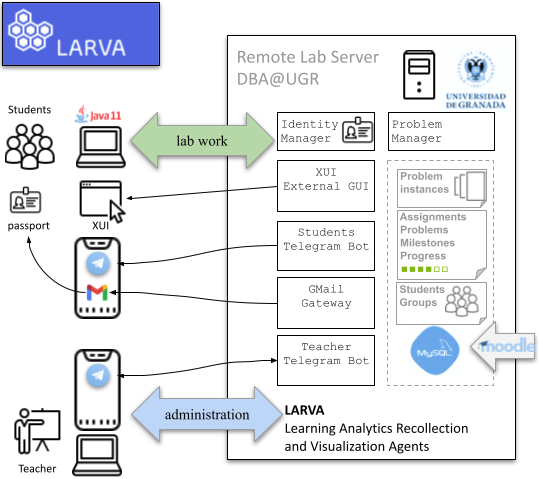
\includegraphics[width=0.60\textwidth]{imagenes/LARVA2122Architecturec.png}
    \caption{Arquitectura del Servidor Remoto}
    \label{fig:architecture}
\end{figure}

\begin{table}[H]
\centering
\caption{Muestra de los datos que se recopilan en el servidor.}
\label{tab:example}
\begin{tabular}{cccccc}
\hline
\textbf{Year} & \textbf{Group} & \textbf{SessionID} & \textbf{Date}       & \textbf{Problem} & \textbf{Step} \\ \hline
1819          & Keid           & 493252533735       & 28/10/2018 20:23:35 & P1               & 1             \\ 
1819          & Keid           & 493252533735       & 28/10/2018 20:23:40 & P1               & 3             \\ 
1819          & Keid           & 389034076811       & 7/11/2018 19:01:49  & P2               & 1             \\
1819          & Cerastes       & 487544594557       & 27/10/2018 13:05:11 & P1               & 1             \\
1819          & Cerastes       & 487544594557       & 27/10/2018 13:10:57 & P1               & 3             \\
1819          & Jabbah         & 550676318711       & 20/12/2018 22:22:42 & P8               & 1             \\
1819          & Cerastes       & 336303012053       & 17/12/2018 13:28:50 & P9               & 1             \\ 
1819          & Keid           & 563159878397       & 25/10/2018 12:41:43 & P8               & 1             \\ \hline
\end{tabular}
\end{table}

\subsection{Los años analizados y los registros existentes}
En total tenemos registros de $7$ años consecutivos (desde el curso académico $1516$ al $2122$), cada uno de los cuáles con los registros y las sesiones de trabajo que se muestran en la Tabla \ref{tab:records}.

\begin{table}[H]
\centering
\caption{Número de registros y sesiones almacenados en el servidor por años.}
\label{tab:records}
\begin{tabular}{ccc}
\hline
\textbf{Year}  & \textbf{Activity Records} & \textbf{Sessions}  \\ \hline
Y2015 & 12088            &  4489  \\
Y2016 & 12525            &  4538  \\
Y2017 & 9088             &  3661  \\
Y2018 & 5705             &  2811  \\
Y2019 & 14475            &  5156  \\
Y2020 & 21188            &  3900  \\
Y2021 & 11961            &  6113  \\ \hline
\end{tabular}
\end{table}

\subsection{El número de grupos cada año}
El número de grupos puede variar en cada curso en función del número de alumnos matriculados en la asignatura ese año. Así pues, se muestran a continuación en las Tablas \ref{tab:groups1} y \ref{tab:groups2} los grupos por curso académico.

\begin{table}[H]
\centering
\caption{Listado de los grupos por curso académico.}
\label{tab:groups1}
\begin{tabular}{cccc}
\hline
\textbf{Y2015} & \textbf{Y2016} & \textbf{Y2017} & \textbf{Y2018} \\ \hline
DBA 1516 P2 GA & DBA 1617 P2 GA & DBA 1718 P2 GA & DBA 1819 P2 GB \\
DBA 1516 P2 GB & DBA 1617 P2 GB & DBA 1718 P2 GB & DBA 1819 P2 GC \\
DBA 1516 P2 GC & DBA 1617 P2 GD & DBA 1718 P2 GC & DBA 1819 P2 GD \\
DBA 1516 P2 GD & DBA 1617 P2 GE & DBA 1718 P2 GD & DBA 1819 P2 GE \\
DBA 1516 P2 GE & DBA 1617 P2 GF & DBA 1718 P2 GE & DBA 1819 P2 GF \\
DBA 1516 P2 GF & DBA 1617 P2 GG & DBA 1718 P2 GG & DBA 1819 P2 GG \\
DBA 1516 P2 GG & DBA 1617 P2 GH & DBA 1718 P2 GH & DBA 1819 P2 GH \\
DBA 1516 P2 GH & DBA 1617 P2 GI & 				 & DBA 1819 P2 GI \\
DBA 1516 P2 GI & DBA 1617 P2 GJ & 				 & DBA 1819 P2 GJ \\
			   &				&			     & DBA 1819 P2 GK \\
			   &				&				 & DBA 1819 P2 GL \\ \hline
\end{tabular}
\end{table}

\begin{table}[H]
\centering
\caption{Listado de los grupos por curso académico.}
\label{tab:groups2}
\begin{tabular}{ccc}
\hline
\textbf{Y2019} & \textbf{Y2020} & \textbf{Y2021} \\ \hline
DBA 1920 P2 GB & DBA 2021 P2 GA & DBA 2122 P2 GA \\
DBA 1920 P2 GC & DBA 2021 P2 GB & DBA 2122 P2 GB \\
DBA 1920 P2 GD & DBA 2021 P2 GC & DBA 2122 P2 GC \\
DBA 1920 P2 GE & DBA 2021 P2 GD & DBA 2122 P2 GD \\
DBA 1920 P2 GF & DBA 2021 P2 GE & DBA 2122 P2 GE \\
DBA 1920 P2 GH & DBA 2021 P2 GF & DBA 2122 P2 GF \\
DBA 1920 P2 GI & DBA 2021 P2 GG & DBA 2122 P2 GG \\
DBA 1920 P2 GJ & DBA 2021 P2 GH & DBA 2122 P2 GH \\
DBA 1920 P2 GK & DBA 2021 P2 GI & DBA 2122 P2 GI \\
DBA 1920 P2 GL & DBA 2021 P2 GJ & DBA 2122 P2 GJ \\
DBA 1920 P2 GM & DBA 2021 P2 GK & DBA 2122 P2 GK \\
DBA 1920 P2 GN & DBA 2021 P2 GL & DBA 2122 P2 GL \\
			   & DBA 2021 P2 GM & DBA 2122 P2 GM \\
			   &         		& DBA 2122 P2 GN \\
			   & 				& DBA 2122 P2 GO \\
			   &				& DBA 2122 P2 GP \\ \hline
\end{tabular}
\end{table}

\subsection{El periodo de tiempo analizado cada año}

En la Tabla \ref{tab:days} se muestra el número de días que dura la práctica cada año. Se puede apreciar una gran diferencia en la duración de la práctica de 2018 respecto a las demás. Esto se debe a que, a petición de los alumnos, se prorrogó la entrega de la práctica hasta casi el final del semestre. Este retraso no supuso un atrasamiento real de los problemas a resolver pues los alumnos fueron capaces de resolverlos en tiempo y forma al menos una vez, y solo se produjo un retraso en la entrega de las versiones definitivas.

\begin{table}[H]
\centering
\caption{Número de días que dura la práctica cada año.}
\label{tab:days}
\begin{tabular}{cc}
\hline
\textbf{Year}  & \textbf{Length (days)}  \\ \hline
Y2015 & 33 \\
Y2016 & 24 \\
Y2017 & 30 \\
Y2018 & 18 \\
Y2019 & 28 \\
Y2020 & 17 \\
Y2021 & 39 \\ \hline
\end{tabular}
\end{table}

\subsection{El conjunto de problemas analizados cada año}

Todos los años hay 9 problemas de dificultad similar que deben ser resueltos por todos los grupos.

Para aproximarnos al concepto subjetivo de ``dificultad del problema'' vamos a analizar el número de sesiones fallidas que necesita cada alumno para resolverlos por primera vez con respecto al número total de sesiones de ese problema (tasa de fallo) y la duración de este periodo en horas.

\subsubsection{Dificultad del problema: la tasa de fallo}

Cada vez que se abre un problema es una sesión de trabajo, la cual puede terminar como fallo (fail) si no se consigue resolver el problema, o éxito (solved) en caso de que se haya resuelto el problema. La tasa de fallo es el cociente entre el número total de sesiones fallidas entre el número total de sesiones de un mismo problema.

\textbf{Falta imagen.}

De hecho, el análisis de la tasa de fallo a lo largo de los problemas detecta distribuciones de probabilidad diferentes (ANOVA p=2e-16, KW p=2.2e-16)

\textbf{Falta tabla.}

Por pares.

\textbf{Falta tabla.}

Intervalos de confianza.

\textbf{Falta imagen.}

Estos datos hay que interpretarlos de manera incremental, pues para resolver un problema Pi requiere las habilidades de Pj(0<=j<i) más habilidades nuevas propias de Pi Periódicamente se incrementa notablemente el nivel de dificultad. P1 es el que más cuesta porque siempre cuesta trabajo empezar, P2-4 son muy parecidos y P5 es un poco más difícil, P6-P8 suben un escalón de dificultad y P9 también.

\subsubsection{Dificultad del problema: tiempo necesario en resolverlo}

Es el número de horas que transcurren desde que el problema se abre por primera vez hasta que es resuelto por primera vez.

\textbf{Falta imagen.}

De nuevo los tests detectan comportamientos diferentes (ANOVA p=9.27e-5, KW p=8.8e-8).

\textbf{Falta tabla.}

Por pares.

\textbf{Falta tabla.}

Intervalos de confianza.

\textbf{Falta imagen.}

Por lo tanto, se puede ver, dadas las evidencias aportadas que la resolución de cada problema exige respuestas claramente diferentes por parte del alumnado.

\subsection{Actividad registrada}

En la Tabla \ref{tab:records} pueden verse las sesiones por año.

Al ser un servicio 24 horas los 7 días de la semana, los alumnos interactúan con el laboratorio remoto en cualquier día de la semana tal y como puede verse en la Figura \ref{fig:days} y a cualquier hora del día (Figura \ref{fig:hours}).

\begin{figure}[H]
    \centering
    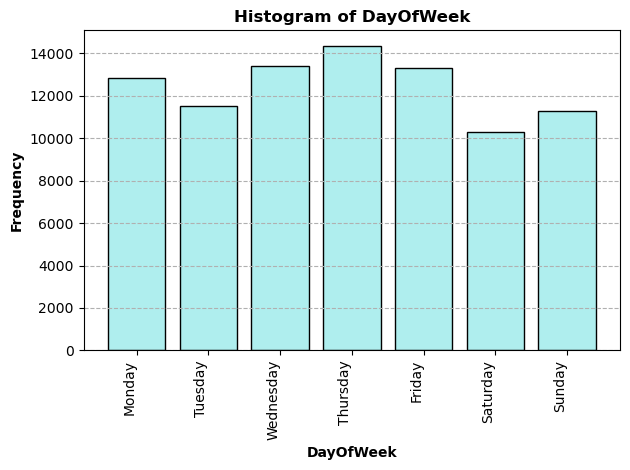
\includegraphics[width=0.80\textwidth]{imagenes/histogramdayofweek.png}
    \caption{Histograma de los días de la semana.}
    \label{fig:days}
\end{figure}

\begin{figure}[H]
    \centering
    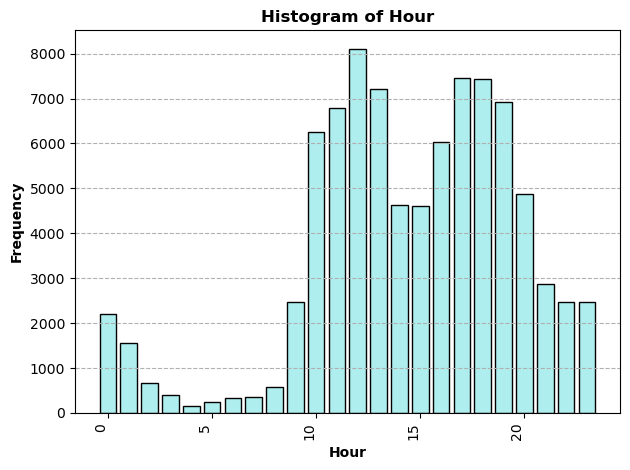
\includegraphics[width=0.80\textwidth]{imagenes/histogramhour.png}
    \caption{Histograma de las horas del día.}
    \label{fig:hours}
\end{figure}

\subsubsection{Número y tipo de sesiones de trabajo}

El número y tipo de las sesiones de trabajo de cada uno de los grupos puede contemplarse en la Tabla \ref{tab:type}.

\begin{longtable}{llrrr}
\hline
\textbf{Year} & \textbf{Group} &  \textbf{fail} &  \textbf{solved} &  \textbf{all} \\
\hline
Y2015 & DBA 1516 P2 GA &   738 &      54 &  792 \\
Y2015 & DBA 1516 P2 GB &    62 &      49 &  111 \\
Y2015 & DBA 1516 P2 GC &   142 &     195 &  337 \\
Y2015 & DBA 1516 P2 GD &   298 &      80 &  378 \\
Y2015 & DBA 1516 P2 GE &   597 &     139 &  736 \\
Y2015 & DBA 1516 P2 GF &   246 &     110 &  356 \\
Y2015 & DBA 1516 P2 GG &   398 &      64 &  462 \\
Y2015 & DBA 1516 P2 GH &   525 &     181 &  706 \\
Y2015 & DBA 1516 P2 GI &   469 &     142 &  611 \\
Y2016 & DBA 1617 P2 GA &   132 &      59 &  191 \\
Y2016 & DBA 1617 P2 GB &   564 &     178 &  742 \\
Y2016 & DBA 1617 P2 GD &   154 &     208 &  362 \\
Y2016 & DBA 1617 P2 GE &   258 &     316 &  574 \\
Y2016 & DBA 1617 P2 GF &   126 &      47 &  173 \\
Y2016 & DBA 1617 P2 GG &   680 &     187 &  867 \\
Y2016 & DBA 1617 P2 GH &   722 &     161 &  883 \\
Y2016 & DBA 1617 P2 GI &   252 &     122 &  374 \\
Y2016 & DBA 1617 P2 GJ &   333 &      39 &  372 \\
Y2017 & DBA 1718 P2 GA &   186 &      46 &  232 \\
Y2017 & DBA 1718 P2 GB &  1282 &     139 & 1421 \\
Y2017 & DBA 1718 P2 GC &   369 &      73 &  442 \\
Y2017 & DBA 1718 P2 GD &   369 &      74 &  443 \\
Y2017 & DBA 1718 P2 GE &   468 &      48 &  516 \\
Y2017 & DBA 1718 P2 GG &   156 &     178 &  334 \\
Y2017 & DBA 1718 P2 GH &   235 &      38 &  273 \\
Y2018 & DBA 1819 P2 GB &   148 &       0 &  148 \\
Y2018 & DBA 1819 P2 GC &   178 &       0 &  178 \\
Y2018 & DBA 1819 P2 GD &   190 &       0 &  190 \\
Y2018 & DBA 1819 P2 GE &   158 &       0 &  158 \\
Y2018 & DBA 1819 P2 GF &   190 &       0 &  190 \\
Y2018 & DBA 1819 P2 GG &   266 &       0 &  266 \\
Y2018 & DBA 1819 P2 GH &   434 &       0 &  434 \\
Y2018 & DBA 1819 P2 GI &   242 &       0 &  242 \\
Y2018 & DBA 1819 P2 GJ &   373 &       0 &  373 \\
Y2018 & DBA 1819 P2 GK &   575 &       0 &  575 \\
Y2018 & DBA 1819 P2 GL &    57 &       0 &   57 \\
Y2019 & DBA 1920 P2 GB &   179 &      71 &  250 \\
Y2019 & DBA 1920 P2 GC &   366 &     116 &  482 \\
Y2019 & DBA 1920 P2 GD &   238 &     110 &  348 \\
Y2019 & DBA 1920 P2 GE &   266 &      63 &  329 \\
Y2019 & DBA 1920 P2 GF &   840 &     271 & 1111 \\
Y2019 & DBA 1920 P2 GH &   206 &      54 &  260 \\
Y2019 & DBA 1920 P2 GI &   119 &      37 &  156 \\
Y2019 & DBA 1920 P2 GJ &   588 &      48 &  636 \\
Y2019 & DBA 1920 P2 GK &   599 &     222 &  821 \\
Y2019 & DBA 1920 P2 GL &   388 &      56 &  444 \\
Y2019 & DBA 1920 P2 GM &   124 &      46 &  170 \\
Y2019 & DBA 1920 P2 GN &   122 &      27 &  149 \\
Y2020 & DBA 2021 P2 GA &   265 &      99 &  364 \\
Y2020 & DBA 2021 P2 GB &   221 &     174 &  395 \\
Y2020 & DBA 2021 P2 GC &   189 &      88 &  277 \\
Y2020 & DBA 2021 P2 GD &   104 &     231 &  335 \\
Y2020 & DBA 2021 P2 GE &    30 &      23 &   53 \\
Y2020 & DBA 2021 P2 GF &   138 &      28 &  166 \\
Y2020 & DBA 2021 P2 GG &   142 &      99 &  241 \\
Y2020 & DBA 2021 P2 GH &   250 &      31 &  281 \\
Y2020 & DBA 2021 P2 GI &   205 &     136 &  341 \\
Y2020 & DBA 2021 P2 GJ &   376 &      82 &  458 \\
Y2020 & DBA 2021 P2 GK &   177 &     105 &  282 \\
Y2020 & DBA 2021 P2 GL &   517 &      93 &  610 \\
Y2020 & DBA 2021 P2 GM &    60 &      37 &   97 \\
Y2021 & DBA 2122 P2 GA &   336 &      48 &  384 \\
Y2021 & DBA 2122 P2 GB &   471 &      28 &  499 \\
Y2021 & DBA 2122 P2 GC &   516 &      39 &  555 \\
Y2021 & DBA 2122 P2 GD &   347 &      34 &  381 \\
Y2021 & DBA 2122 P2 GE &   168 &      23 &  191 \\
Y2021 & DBA 2122 P2 GF &   418 &      37 &  455 \\
Y2021 & DBA 2122 P2 GG &   331 &      37 &  368 \\
Y2021 & DBA 2122 P2 GH &   258 &      45 &  303 \\
Y2021 & DBA 2122 P2 GI &   490 &      59 &  549 \\
Y2021 & DBA 2122 P2 GJ &   273 &      30 &  303 \\
Y2021 & DBA 2122 P2 GK &   425 &      39 &  464 \\
Y2021 & DBA 2122 P2 GL &   232 &      19 &  251 \\
Y2021 & DBA 2122 P2 GM &   513 &      39 &  552 \\
Y2021 & DBA 2122 P2 GN &   169 &      18 &  187 \\
Y2021 & DBA 2122 P2 GO &   359 &      40 &  399 \\
Y2021 & DBA 2122 P2 GP &   262 &      10 &  272 \\
\hline
\caption{Número y tipo de las sesiones de trabajo.}
\label{tab:type}
\end{longtable}

\textbf{Análisis de la normalidad de distribución del número de sesiones}

% latex table generated in R 4.3.0 by xtable 1.8-4 package
% Mon May 22 23:29:03 2023
\begin{table}[H]
\centering
\begin{tabular}{lrrrrr}
  \hline
 & Df & Sum Sq & Mean Sq & F value & Pr($>$F) \\ 
  \hline
ndsp[[nVariable]] & 6 & 666498.27 & 111083.05 & 2.11 & 0.0630 \\ 
  Residuals         & 70 & 3688035.44 & 52686.22 &  &  \\ 
   \hline
\end{tabular}
\end{table}

% latex table generated in R 4.3.0 by xtable 1.8-4 package
% Mon May 22 23:33:01 2023
\begin{table}[H]
\centering
\begin{tabular}{rrrrr}
  \hline
 & diff & lwr & upr & p adj \\ 
  \hline
Y2016-Y2015 & 5.44 & -323.03 & 333.92 & 1.00 \\ 
  Y2017-Y2015 & 24.22 & -326.93 & 375.38 & 1.00 \\ 
  Y2018-Y2015 & -243.23 & -556.42 & 69.96 & 0.23 \\ 
  Y2019-Y2015 & -69.11 & -376.37 & 238.15 & 0.99 \\ 
  Y2020-Y2015 & -198.78 & -500.93 & 103.38 & 0.43 \\ 
  Y2021-Y2015 & -116.72 & -407.05 & 173.62 & 0.88 \\ 
  Y2017-Y2016 & 18.78 & -332.38 & 369.93 & 1.00 \\ 
  Y2018-Y2016 & -248.68 & -561.87 & 64.51 & 0.21 \\ 
  Y2019-Y2016 & -74.56 & -381.82 & 232.71 & 0.99 \\ 
  Y2020-Y2016 & -204.22 & -506.38 & 97.93 & 0.39 \\ 
  Y2021-Y2016 & -122.16 & -412.49 & 168.18 & 0.86 \\ 
  Y2018-Y2017 & -267.45 & -604.35 & 69.45 & 0.21 \\ 
  Y2019-Y2017 & -93.33 & -424.73 & 238.06 & 0.98 \\ 
  Y2020-Y2017 & -223.00 & -549.67 & 103.67 & 0.38 \\ 
  Y2021-Y2017 & -140.94 & -456.70 & 174.83 & 0.82 \\ 
  Y2019-Y2018 & 174.12 & -116.74 & 464.98 & 0.54 \\ 
  Y2020-Y2018 & 44.45 & -241.01 & 329.92 & 1.00 \\ 
  Y2021-Y2018 & 126.52 & -146.40 & 399.44 & 0.80 \\ 
  Y2020-Y2019 & -129.67 & -408.61 & 149.28 & 0.79 \\ 
  Y2021-Y2019 & -47.60 & -313.70 & 218.49 & 1.00 \\ 
  Y2021-Y2020 & 82.06 & -178.12 & 342.24 & 0.96 \\ 
   \hline
\end{tabular}
\end{table}

\begin{figure}[H]
    \centering
    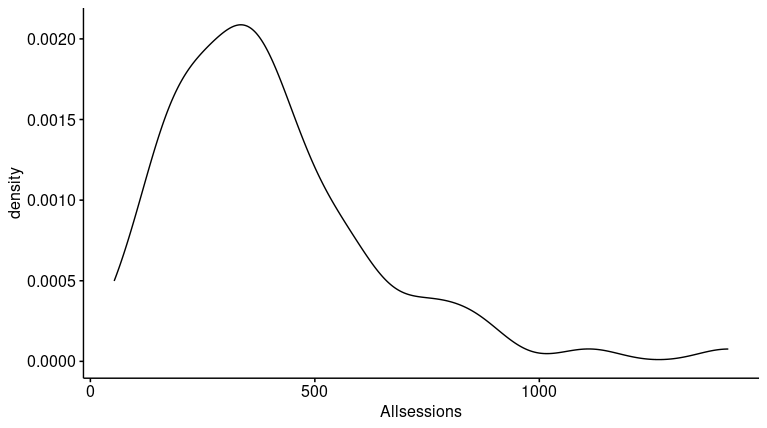
\includegraphics[width=0.75\textwidth]{imagenes/allsessions/Rplot04.png}
    \caption{Función de densidad de probabilidad del número de sesiones.}
    \label{fig:densitysessions}
\end{figure}

\begin{figure}[H]
    \centering
    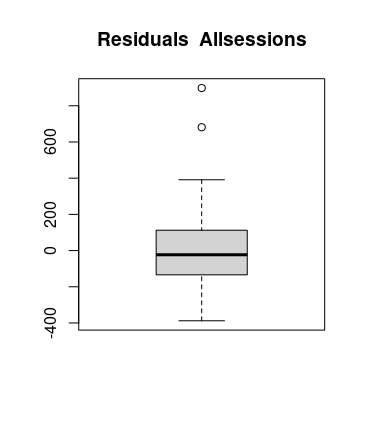
\includegraphics[width=0.50\textwidth]{imagenes/allsessions/Rplot02.png}
    \caption{Boxplot de los residuos del número de sesiones.}
    \label{fig:boxplotresiduals}
\end{figure}

\begin{figure}[H]
    \centering
    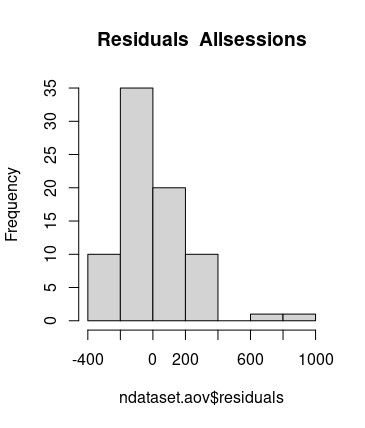
\includegraphics[width=0.50\textwidth]{imagenes/allsessions/Rplot03.png}
    \caption{Histograma de los residuos del número de sesiones.}
    \label{fig:histogramresiduals}
\end{figure}


\begin{figure}[H]
    \centering
    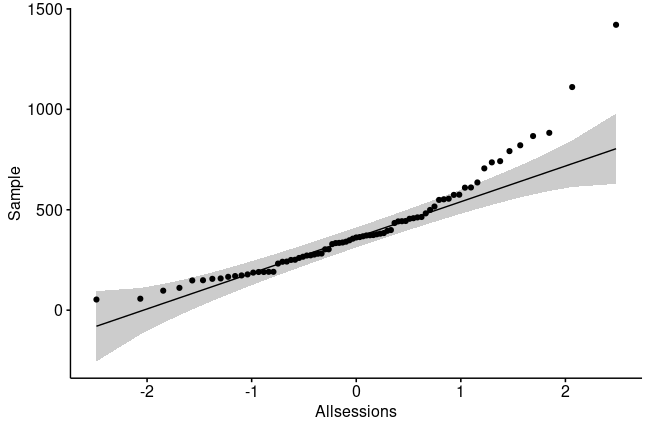
\includegraphics[width=0.75\textwidth]{imagenes/allsessions/Rplot05.png}
    \caption{Gráfico Q-Q del número de sesiones.}
    \label{fig:q-qsessions}
\end{figure}

La distribución no es perfectamente normal pero es casi-normal si eliminaremos algunos outsiders

\textbf{Sesiones por cada problema}

La principal diferencia en las sesiones abiertas respecto al problema P1 y restantes se deben a que los alumnos utilizan P1 como base de todos los experimentos y para testear las comunicaciones con el servidor por lo que es frecuentemente utilizado, no ya sólo al comienzo, sino durante toda la práctica.

\begin{figure}[H]
    \centering
    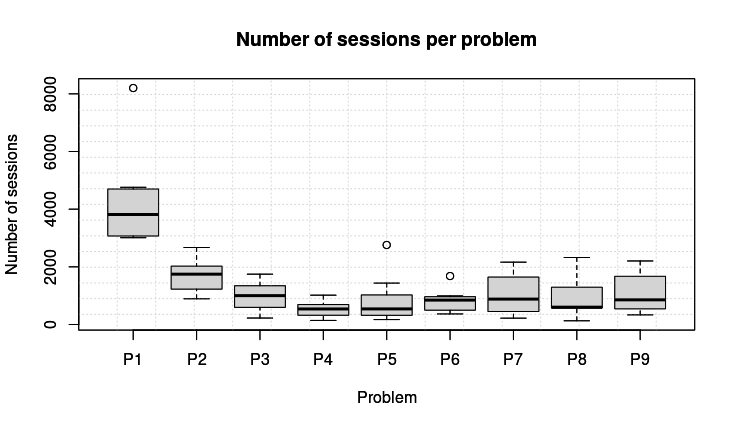
\includegraphics[width=0.85\textwidth]{imagenes/allsessions/Rplot06.png}
    \caption{Boxplot del número de sesiones por problema.}
    \label{fig:boxplotsessionsproblem}
\end{figure}


\textbf{Sesiones cada año}

Lo cierto  es que el análisis detallado de las sesiones de trabajo abiertas en el servidor año tras año, parecen seguir la misma distribución de probabilidad.

\begin{figure}[H]
    \centering
    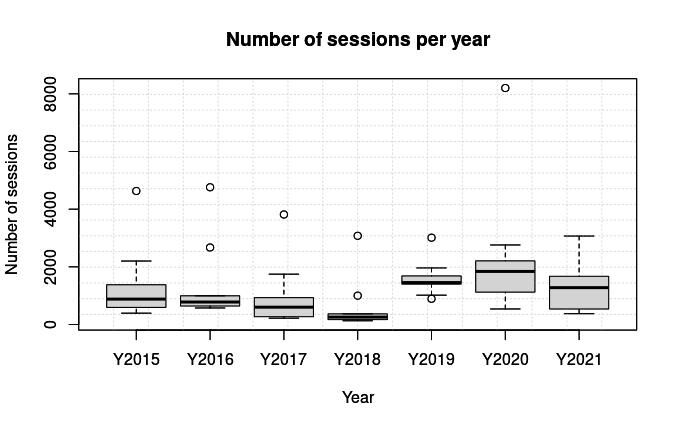
\includegraphics[width=0.80\textwidth]{imagenes/allsessions/Rplot07.png}
    \caption{Boxplot del número de sesiones por año.}
    \label{fig:boxplotsessionsproblem}
\end{figure}

En este caso, ANOVA p=0.103, pero KW p=3.01e-5. Para resolver la discrepancia, se hace un test de Tukey por pares de años en el que se observa que, si bien hay algunos pares un poco justos (p<0.2) casi todos están muy altos.

% latex table generated in R 4.3.0 by xtable 1.8-4 package
% Wed May 24 15:16:22 2023
\begin{table}[ht]
\centering
\begin{tabular}{lrrrrr}
  \hline
 & Df & Sum Sq & Mean Sq & F value & Pr($>$F) \\ 
  \hline
mdsp[[mVariable]] & 6 & 15291674.54 & 2548612.42 & 1.40 & 0.2298 \\ 
  Residuals         & 56 & 101747678.89 & 1816922.84 &  &  \\ 
   \hline
\end{tabular}
\end{table}

% latex table generated in R 4.3.0 by xtable 1.8-4 package
% Wed May 24 15:17:46 2023
\begin{table}[ht]
\centering
\begin{tabular}{rrrrr}
  \hline
 & diff & lwr & upr & p adj \\ 
  \hline
Y2016-Y2015 & 48.56 & -1894.57 & 1991.68 & 1.00 \\ 
  Y2017-Y2015 & -333.33 & -2276.46 & 1609.79 & 1.00 \\ 
  Y2018-Y2015 & -709.22 & -2652.35 & 1233.90 & 0.92 \\ 
  Y2019-Y2015 & 265.22 & -1677.90 & 2208.35 & 1.00 \\ 
  Y2020-Y2015 & 1011.11 & -932.01 & 2954.24 & 0.69 \\ 
  Y2021-Y2015 & -14.11 & -1957.24 & 1929.01 & 1.00 \\ 
  Y2017-Y2016 & -381.89 & -2325.01 & 1561.24 & 1.00 \\ 
  Y2018-Y2016 & -757.78 & -2700.90 & 1185.35 & 0.89 \\ 
  Y2019-Y2016 & 216.67 & -1726.46 & 2159.79 & 1.00 \\ 
  Y2020-Y2016 & 962.56 & -980.57 & 2905.68 & 0.73 \\ 
  Y2021-Y2016 & -62.67 & -2005.79 & 1880.46 & 1.00 \\ 
  Y2018-Y2017 & -375.89 & -2319.01 & 1567.24 & 1.00 \\ 
  Y2019-Y2017 & 598.56 & -1344.57 & 2541.68 & 0.96 \\ 
  Y2020-Y2017 & 1344.44 & -598.68 & 3287.57 & 0.36 \\ 
  Y2021-Y2017 & 319.22 & -1623.90 & 2262.35 & 1.00 \\ 
  Y2019-Y2018 & 974.44 & -968.68 & 2917.57 & 0.72 \\ 
  Y2020-Y2018 & 1720.33 & -222.79 & 3663.46 & 0.12 \\ 
  Y2021-Y2018 & 695.11 & -1248.01 & 2638.24 & 0.93 \\ 
  Y2020-Y2019 & 745.89 & -1197.24 & 2689.01 & 0.90 \\ 
  Y2021-Y2019 & -279.33 & -2222.46 & 1663.79 & 1.00 \\ 
  Y2021-Y2020 & -1025.22 & -2968.35 & 917.90 & 0.67 \\ 
   \hline
\end{tabular}
\end{table}

\begin{figure}[H]
    \centering
    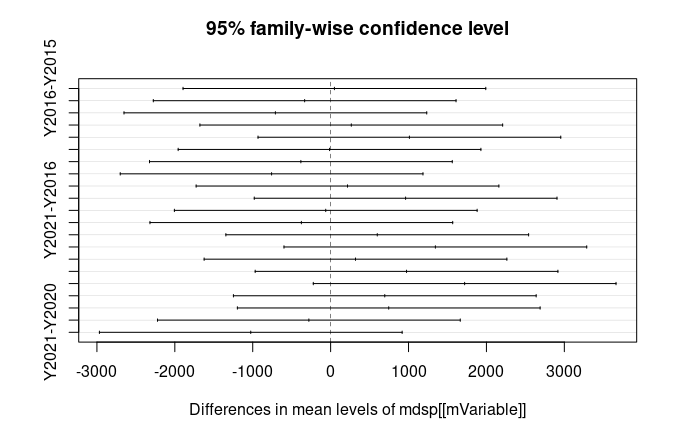
\includegraphics[width=0.80\textwidth]{imagenes/allsessions/Rplot08.png}
    \caption{Intervalos de confianza del número de sesiones por año.}
    \label{fig:confidence}
\end{figure}